In the first prototypes, TRITIUM-IFIC 0 and TRITIUM-IFIC-1, the fibers were directly coupled to the photosensor, so the detected photons were only those guided by fibers. However, in the last prototypes, TRITIUM-Aveiro and TRITIUM-IFIC 2, two PMMA windows are used, which allows the detection of photons guided by fiber and photons that come from the water medium.

To quantify the importance of this effect, the TRITIUM-Aveiro prototype was simulated and the distribution of the number of photons that reach the PMMA per tritium event are shown in Figure \ref{fig:PMMAEffect}. Fiber-guided photons are shown in a red distribution, while those traveling in the water medium are represented in the blue histogram.

\begin{figure}[hbtp]
\centering
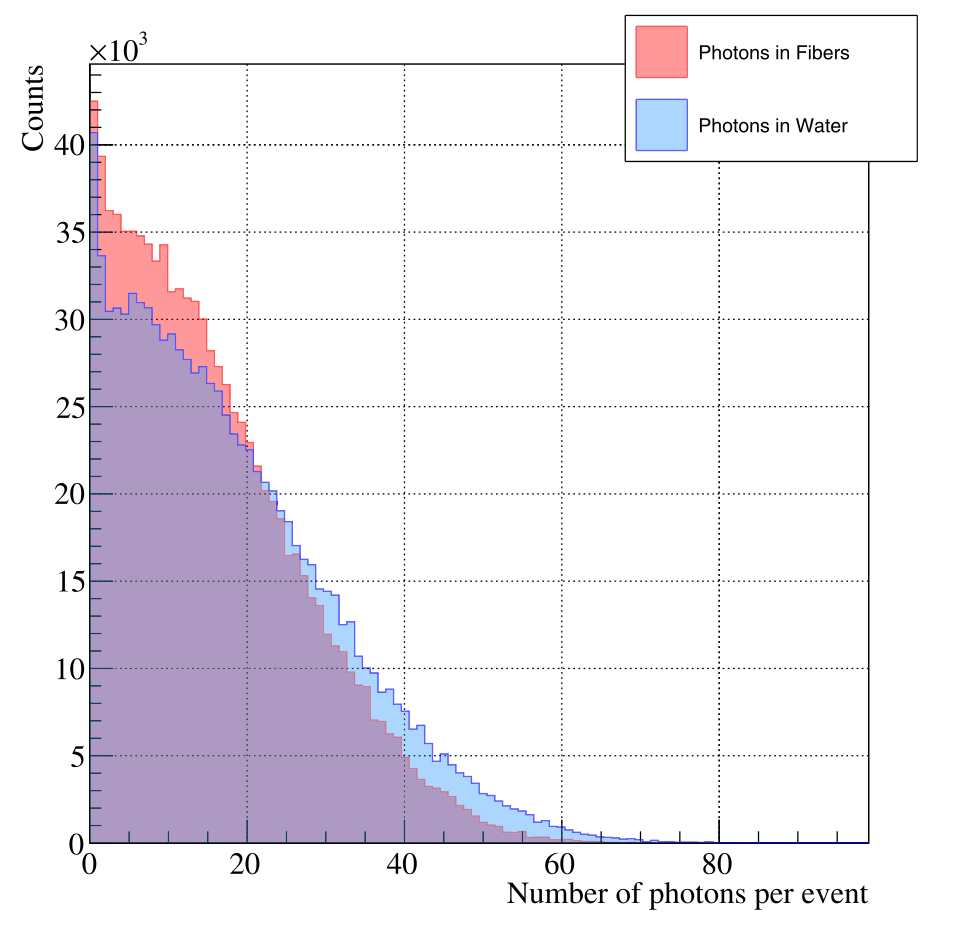
\includegraphics[scale=0.3]{Figures/8SimulationsResults/81TRITIUMDesign/815PMMA/PhotonsDetectedWaterFiber.png}
\caption{Distribution of photons reaching PMMA windows. The red histogram includes those guided by fibers and the blue histogram includes those traveling in the water medium \cite{SimulationPaperCarlos}.\label{fig:PMMAEffect}}
\end{figure}

It can be seen that the tritium signal obtained from the water is as important as that obtained from the fibers, contributing half of a signal. Therefore, an improvement in tritium detection efficiency is achieved using PMMA windows.